\section{Аналитический раздел}

В данном разделе будет проведен анализ предметной области анализа структуры документов, будет приведена формализация задачи предметной области, будут описаны существующие методы и алгоритмы, будет проведена классификация существующих методов, будет обоснована потребность в разработке нового метода, будет сформулирована цель данной работы и формализована постановка задачи.

% NOTE:
% Анализ предметной области + выделяется основной объект исследования
% Формализовать предметную область с помощью IDEF0 модели, если сложно с помощью мат формул
% Затем выполняется обзор существующих методов и алгоритмов решения идентифицированной проблемы предметной области (со ссылками на научные статьи), анализируются достоинства и недостатки каждого из них
% Результаты проведенного анализа классифицируются и оформляются в табличной форме
% На основе выполненного анализа обосновывается необходимость разработки или адаптации существующего метода или алгоритма
% Одним из основных выводов аналитического раздела должно стать формализованное описание проблемы предметной области, на решение которой будет направлен проект, включающее в себя
% - описание входных и выходных данных
% - указание ограничений, в рамках которых будет разработан новый метод или алгоритм
% - описание способов тестирования разработанного метода
% - описание функциональных требований к разрабатываемому ПО

% NOTE:
% Если в результате работы будет создано ПО, реализующее большое количество типичных способов взаимодействия с пользователем, необходимо каждый из этих способов описать с помощью диаграммы прецедентов

% Рек. Объем 25-30 страниц

\subsection{Анализ предметной области}

В данном подразделе будет проведен анализ предметной области анализа структуры документов, будут рассмотрены существующие типы макетов документов, будут описаны структура научно-технического текста и его составные части.

% Предметная область анализа структуры документов
% Описать процесс анализа структуры документов
% Описать существующие типы макетов документов
% Описать структуру научного текста

\subsubsection{Анализ структуры документов}

Анализ структуры документов (Document layout analysis, DLA) --- процесс сегментирования входного изображения документа на однородные компоненты, такие как блоки текста, рисунки, таблицы, графики и т.д., и их классификации~\cite{tnt}.

В общем случае анализ структуры документа делится на два взаимосвязанных процесса: физический и логический анализ.
Целью физического анализа является выявление структуры документа и определение границ его однородных областей.
Целью логического анализа является разметка обнаруженных областей. Выявленные области классифицируются как элементы документа --- рисунки, заголовки, абзацы, логотипы, подписи и другие.~\cite{dla-survey}

Процесс анализа структуры документов состоит из двух основных этапов --- этапа предварительной обработки и этапа анализа макета документа~\cite{dla-survey, dla-book}.

\newpage

На рисунке ниже приведена схема процесса анализа структуры документов.

\begin{figure}[H]
	\centering
	% 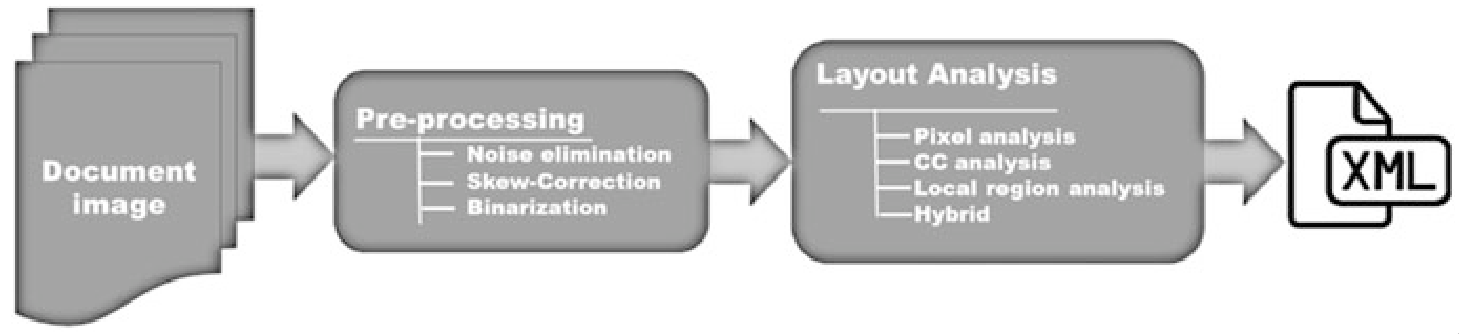
\includegraphics[width=\textwidth]{img/typical-dla-system.png}
	
\includegraphics[width=\textwidth]{diag/dla.pdf}
	\caption{Схема процесса анализа структуры документов~\cite{dla-book}}
	\label{fig:}
\end{figure}

\subsubsection*{Этап предварительной обработки}

Этап анализа макета документа в любом методе анализа структуры документов (далее DLA) часто основывается на определённых предположениях о входных изображениях, таких как отсутствие шума, бинаризация, отсутствие наклона текста или все перечисленные факторы~\cite{dla-survey, dla-book}.

Цель этапа предварительной обработки --- преобразовать входное изображение в соответствии с требованиями этапа анализа макета документа конкретного метода~\cite{dla-survey, dla-book}.

В общем случае на этом этапе используются одна или несколько процедур предварительной обработки, таких как бинаризация, выравнивание и улучшение изображения~\cite{dla-survey, primer}.

\subsubsection*{Этап анализа макета документа}

Анализ макета документа включает в себя определение границ и типов составляющих областей входного изображения документа.
Процесс определения границ областей документа называется сегментацией областей документа, а классификация найденных областей по их типу --- классификацией областей документа.~\cite{dla-book}

Существуют три типа стратегий анализа макета документа: снизу вверх (bottom-up), сверху вниз (top-down) и гибридная (hybrid).

По стратегии снизу вверх (bottom-up) параметры анализа часто вычисляются на основе исходных данных.
Анализ макета документа начинается с небольших элементов, таких как пиксели или связанные компоненты.
Затем однородные элементы объединяются, создавая более крупные области.
Процесс продолжается, пока не будут достигнуты заранее определённые условия остановки.

По стратегии сверху вниз (top-down) анализ макета документа начинается с крупных областей, например, на уровне всего документа.
Затем эта большая область разбивается на более мелкие, такие как колонки текста, на основе определённых правил однородности.
Анализ сверху вниз прекращается, когда дальнейшее разбиение областей становится невозможным или достигаются условия остановки.

Гибридная стратегия (hybrid) представляет собой комбинацию обеих стратегий (снизу вверх и сверху вниз).~\cite{dla-survey}

После сегментации областей происходит их классификация с помощью различных алгоритмов, в результате чего формируется логическая структура документа.

По завершении данного этапа извлеченные геометрическая и логическая структуры сохраняются для последующей реконструкции.
Для этого, как правило, используется иерархическая древовидная структура данных.~\cite{dla-book}

\newpage

\subsubsection{Типы макетов документов}

% Какие есть виды макетов, двухколоночные и т.д.
% Какие используются в научных статьях

Макеты документов могут иметь различные структуры.
Печатные документы можно разделить на шесть типов~\cite{kise}: прямоугольные, Манхэттенские, не-Манхэттенские, многоколоночные Манхэттенские, с горизонтальным наложением и с диагональным наложением.

\begin{figure}[H]
	\centering
    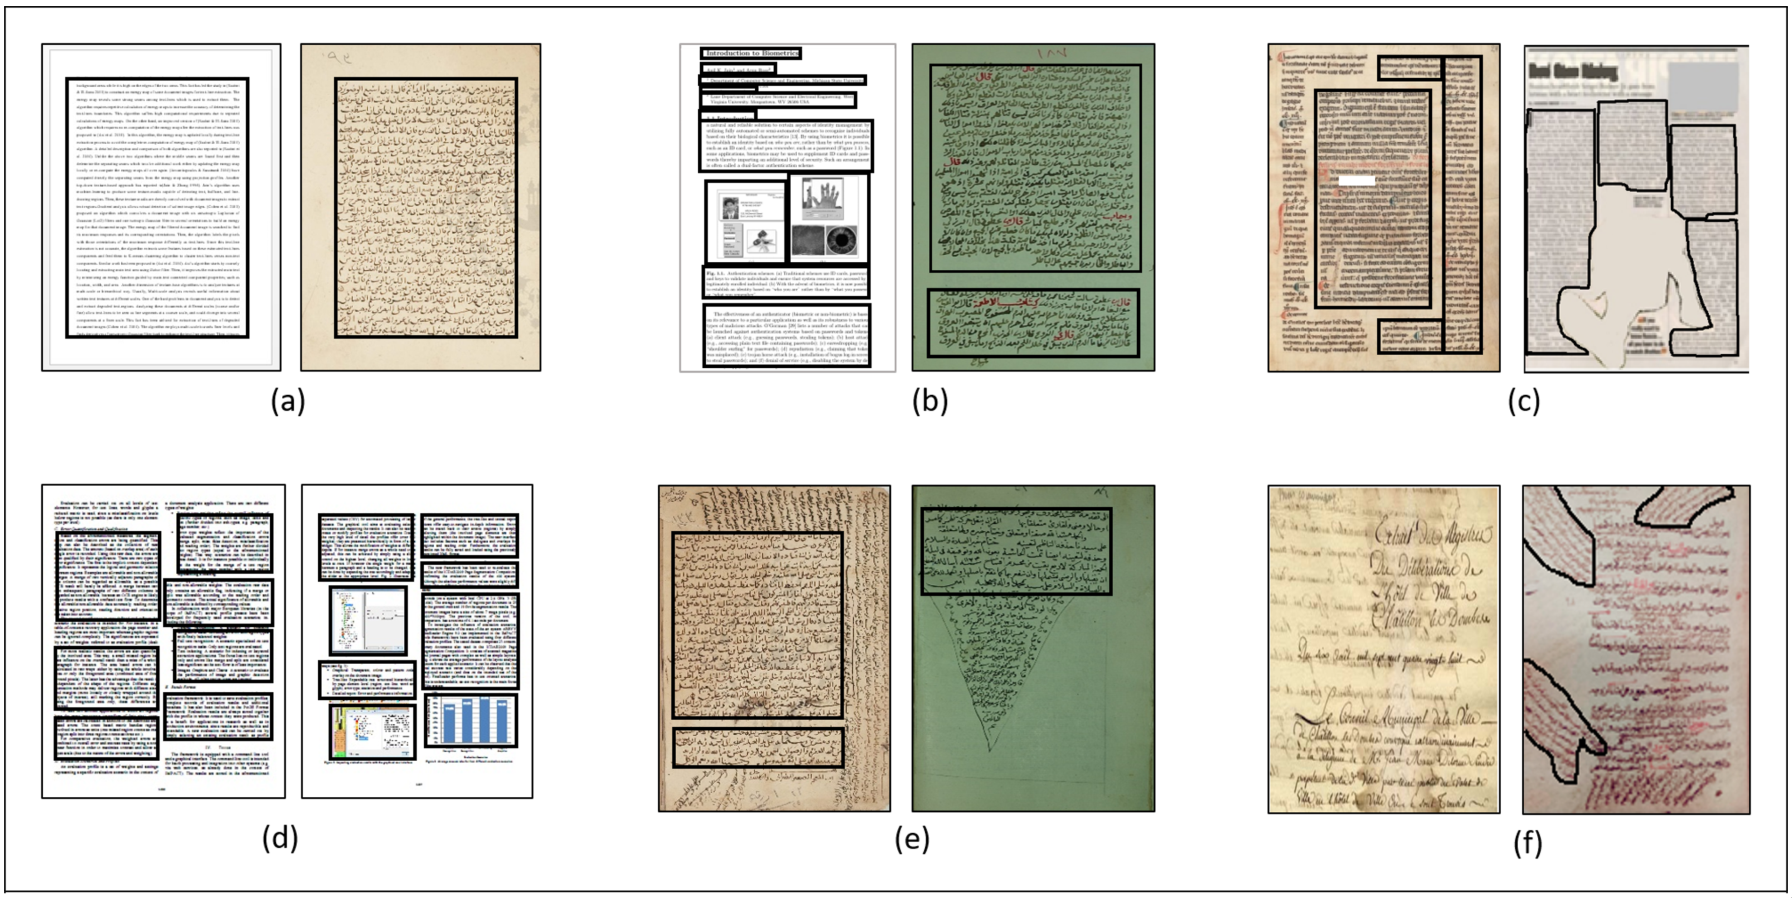
\includegraphics[width=\textwidth]{img/layouts.png}
    \caption{Макеты документов: (a) Стандартный (прямоугольный), (b) Манхэттенский, (c) Не-Манхэттенский, (d) Многоколоночный Манхэттенский, (e) Произвольный (сложный), (f) С горизонтальным и диагональным наложением.~\cite{dla-survey}}
	\label{fig:layouts}
\end{figure}

На рисунке выше показаны примеры описанных типов макетов документов:
\begin{itemize}
    \item Стандартный макет характеризуется большими прямоугольными текстовыми блоками, расположенными в одной или нескольких колонках, при этом каждая колонка содержит по одному абзацу.
    \item Если документ содержит несколько абзацев в колонках, его можно отнести к Манхэттенскому макету.
Примеры таких документов --- научно-технические статьи, журналы и другие.
    \item Не-Манхэттенские макеты включают зоны непрямоугольной формы.
    \item Макеты с наложением содержат элементы, такие как текст, который перекрывает другие элементы документа.
Наложение может возникать, например, из-за просвечивания (см. Рисунок \ref{fig:layouts}(f)).
    \item Документы с произвольными (или сложными) макетами могут включать рукописный и/или печатный текст, содержащий различные стили, типы и размеры шрифтов.
\end{itemize}

Таким образом, документы, содержащие научно-технические тексты, обычно используют Манхэттенский макет.

\subsubsection{Структура научно-технического текста}

Научно-технический текст обычно~\cite{butenko2022, romanov2014, raitskaya2019} следует четко определенному шаблону и имеет следующую структуру:
\begin{enumerate}
    \item Название;
    \item Информация об авторах;
    \item Аннотация и ключевые слова;
    \item Введение;
    \item Основная часть (кроме текста содержащая в том числе таблицы, рисунки, графики, листинги);
    \item Заключение;
    \item Ссылки на литературу.
\end{enumerate}

Содержимое научного текста часто не ограничивается текстом, а содержит также следующие составные части:
\begin{enumerate}
    \item Таблицы;
    \item Листинги;
    \item Схемы алгоритмов;
    \item Рисунки;
    \item Графики.
\end{enumerate}

% На рисунке ниже показана структура научной статьи.
%
% \begin{figure}[H]
% 	\centering
% 	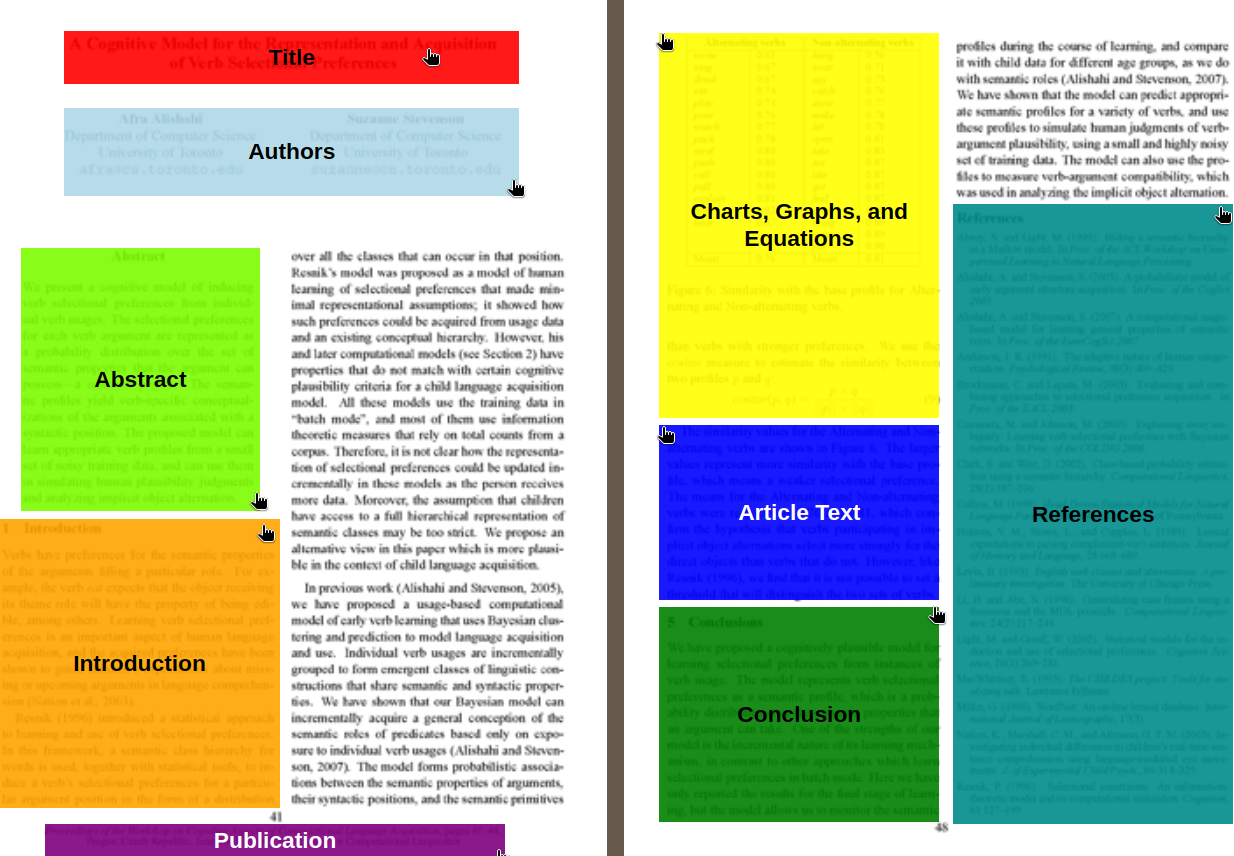
\includegraphics[width=\textwidth]{img/struct-parts-named.png}
% 	\caption{Структура научной статьи}
% 	\label{fig:}
% \end{figure}

Зная структуру научного текста и его основные части можно перейти к формализации задачи выделения составных частей научного текста.

\subsection{Формализация предметной области}

Пусть $ D $ --- документ, представленный в виде набора изображений, содержащих текст, листинги, таблицы, рисунки и прочие структурные элементы.

Документ
\begin{equation}
    D = \{ P_1, P_2 , \dots, P_n \}
    \label{eq:d}
\end{equation}
состоит из страниц $ P_1, P_2, \dots, P_n $, а каждая страница $ P_i $ в свою очередь состоит из множества сегментов $ S_{i,1}, S_{i,2}, \dots, $ $S_{i,m} $.

Сегмент $S_{i,j}$ --- кортеж $(x_{i,j}, y_{i,j}, w_{i,j}, h_{i,j})$, где $(x_{i,j}, y_{i,j})$ --- координаты верхнего левого угла, $w_{i,j}$ --- ширина, $h_{i,j}$ --- высота сегмента.

Требуется построить отображение
\begin{equation}
    F : D \to \{(S_{i,j}, C_{i,j})\},
    \label{eq:f}
\end{equation}
где каждому сегменту $S_{i,j}$ ставится в соответствие класс
\begin{equation}
    C_{i,j} = C_{i,j}(S_{i,j}),
    \label{eq:c}
\end{equation}
область допустимых значений которого определяется согласно требованиям к разметке.

Например, в случае задачи выделения составных частей научного текста, $C_{i,j} \subseteq$ $\{${Фон, Текст, Таблица, Листинг, Схема алгоритма, Рисунок, График, Неопределенность}$\}$;
Сегмент классифицируется как <<Неопределенность>> в случае, когда не удалось распределить его ни в один из предыдущих классов.

Поставленную задачу можно решить, разбив на две подзадачи и решив каждую подзадачу соответственно: первая подзадача --- нахождение сегментов на страницах, вторая подзадача --- классификация найденных сегментов (определение $C_{i,j}$ для каждого объекта $S_{i,j}$).

Решением первой подзадачи является построение отображений
\begin{equation}
    P_i \to \{ S_{i,j} \},
    \label{eq:p}
\end{equation}
решением второй подзадачи является построение отображений
\begin{equation}
    S_{i,j} \to C_{i,j}.
    \label{eq:o}
\end{equation}

Далее будут рассмотрены существующие методы, позволяющие решить поставленную задачу.

\subsection{Описание существующих методов}

% Описать существующие методы анализа структуры документов

В данном подразделе будет описана суть методов на основе анализа связных компонент, методов на основе анализа проекционного профиля, алгоритма размазывания по длине серии, методов на основе машинного обучения и гибридных методов на основе анализа проекционного профиля и анализа связных компонент.

\subsubsection{Анализ связных компонент}

Методы на основе связных компонент (Connected Component Analysis, CCA) анализируют и объединяют связные компоненты для формирования однородных областей.

Определение начальных компонент, которые впоследствии объединяются, происходит, как правило, следующим образом.
Изображение проходит стадию бинаризации (преобразование к черно-белому формату и назначение каждому пикселю интенсивности 0 или 1), после чего смежные пиксели объединяются на основе 4- или 8-связности.
При 4-связности два пикселя считаются связными, если они расположены друг за другом по горизонтали или вертикали.
При 8-связности два пикселя считаются связными, если они являются 4-связными, либо расположены друг за другом по диагонали.

После определения начальных компонент, компоненты объединяются в однородные области путем применения специальных алгоритмов.
В качестве таких алгоритмов могут выступать, например, преобразование Хафа (Hough transform) или алгоритм K-ближайших соседей (K-nearest neighbor, KNN)~\cite{dla-book}.

Далее происходит классификация однородных областей.
Для классфикации области могут использоваться эвристические алгоритмы (классификация на основе ширины штриха, размера или формы компонента) и алгоритмы на основе машинного обучения.

Методы на основе связных компонент могут работать в условиях скошенного текста при условии, что межстрочный интервал меньше пробела между абзацами~\cite{dla-book}.

\subsubsection{Анализ проекционного профиля}

Суть методов на основе анализа проекционного профиля (Projection Profile Analysis, PPA) заключается в следующем.
Пиксели документа проецируются на вертикальную и горизонтальную ось, после чего строятся гистограммы распределения пикселей.
Далее анализируются пики и впадины на гистограммах.
Впадины на вертикальном профиле указывают на пробелы между колонками текста.
Впадины на горизонтальном профиле указывают на пробелы между строками или блоками текста.

На основе проведенного анализа можно разделить документ на логические компоненты --- текстовые блоки, заголовки, таблицы, изображения.

Данные методы работают только с Манхэттенскими макетами документов и чувствительны ко скошенности текста в документе~\cite{dla-book}.

\newpage

\subsubsection{Алгоритм размазывания по длине серии}

Методы на основе RLSA преобразуют бинарное изображение документа путем <<размазывания>> черных пикселей горизонтально и/или вертикально для формирования однородных областей.

На рисунке ниже можно видеть пример работы RLSA.

\begin{figure}[H]
	\centering
	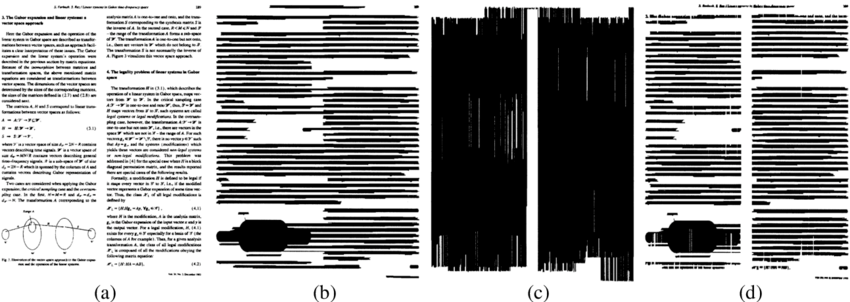
\includegraphics[width=\textwidth]{img/rlsa.png}
    \caption{Пример работы алгоритма RLSA. К начальному изображению документа (a) применяется горизонтальный (b) и вертикальный (c) RLSA, после чего в результате применения операции И к изображениям (b) и (c) формируется (d)}
	\label{fig:}
\end{figure}

Для классификации полученных областей также используются эвристические алгоритмы и алгоритмы на основе машинного обучения.

Данные методы, как и методы на основе анализа проекционного профиля, работают преимущественно с Манхэттенскими макетами документов и чувствительны к скошенному тексту~\cite{dla-book}.

\subsubsection{Методы на основе машинного обучения}

Методы, не основанные на глубоком обучении, используют простые архитектуры нейросетей для обучения.
Анализ с использованием нейросети происходит на трех уровнях: уровне пикселей, уровне блоков текста и уровне страниц.

Методы на основе машинного обучения в области анализа макетов документов страдают от несбалансированности данных и отсутствия контекстной информации.
Если модель обучалась на документах, в наборе данных для обучения количество текстовой и фоновой информации сильно превосходит количество информации о рисунках и графиках.
В связи с этим обученная модель может склоняться в сторону текстовых или фоновых пикселей.~\cite{dla-survey}

Обучение моделей лишь на основе информации о пикселях чревато потерей контекстной информации.
Поэтому при обучении на уровнях блоков текста и страниц прибегают к использованию методов извлечения признаков для создания более надежных моделей.~\cite{dla-survey}

%\subsection{Методы на основе глубокого обучения}
Методы на основе машинного обучения работают с любыми макетами документов и не чувствительны к скошенному тексту.

\subsubsection{Гибридные методы на основе PPA и CCA}

Гибридные методы на основе анализа проекционного профиля и связных компонент используют работают следующим образом.
Начальные компоненты определяются применением метода из PPA, после чего происходит их уточнение применением методов из CCA.

Такой комбинированный подход позволяет лучше сегментировать текст, чем каждый метод по отдельности.

\subsection{Классификация существующих методов}

% Сравнить известные методы анализа структуры документов

Для сравнения рассмотренных методов можно выделить следующие критерии:
\begin{itemize}
    \item Стратегия анализа макета документа;
    \item Скорость работы --- время, необходимое методу для обработки документа и получения результата разметки;
    \item Гибкость --- способность метода адаптироваться к различным типам макетов документов;
    \item Устойчивость --- способность метода адаптироваться к шумам и искажениям текста;
    \item Специальное требование --- позволяет сегментировать не только текст, но и такие составные части научного текста, как таблицы, листинги, схемы, рисунки, графики и прочее.
\end{itemize}

Ниже приведена таблица со сравнительным анализом рассмотренных методов.

\begin{table}[H]
    \centering
    \caption{Классификация методов DLA}
    \label{tab:table}
    \begin{tabular}{|c|c|c|c|c|c|}
        \hline
        \textbf{Метод} & \textbf{Стратегия} & \textbf{Скорость} & \textbf{Гибкость} & \textbf{Ус-ть} & \textbf{СпецТреб} \\ \hline
        CCA        & Снизу вверх & 2 & 2 & 3 & Нет \\ \hline
        PPA        & Сверху вниз & 2 & 3 & 3 & Нет \\ \hline
        RLSA       & Сверху вниз & 1 & 3 & 3 & Нет \\ \hline
        ML         & Снизу вверх & 3 & 1 & 1 & Да \\ \hline
        PPA + CCA  & Гибридный   & 2 & 3 & 2 & Нет \\ \hline
    \end{tabular}
\end{table}

Как можно видеть по сравнительной таблице, ни один из рассмотренных методов не позволяет <<быстро>>, на основе лишь различных эвристик, произвести разметку документа, сегментирующую не только текст, но и другие составные части научного текста.

\newpage

\subsection{Формализованная постановка задачи}

% Сформулировать цель и формализовать постановку задачи в виде функциональной модели

Целью данной работы является разработка метода, позволяющего выделять составные части научного текста на основе простых правил, без использования нейросетей, а также разработка алгоритма, реализующего данный метод.

Формализованная в виде IDEF0 диаграммы постановка задачи представлена на рисунке \ref{fig:a0} ниже.

\begin{figure}[H]
	\centering
	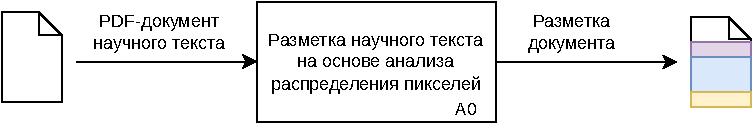
\includegraphics[width=\textwidth]{diag/a0-pres.pdf}
	\caption{Постановка задачи}
	\label{fig:a0}
\end{figure}

\subsection*{Вывод}

В данном разделе был проведен анализ предметной области анализа структуры документов, была приведена формализация задачи предметной области, были описаны существующие методы и алгоритмы, была проведена классификация существующих методов, была обоснована потребность в разработке нового метода, была сформулирована цель данной работы и формализована постановка задачи.
